\usetikzlibrary{arrows.meta,calc}
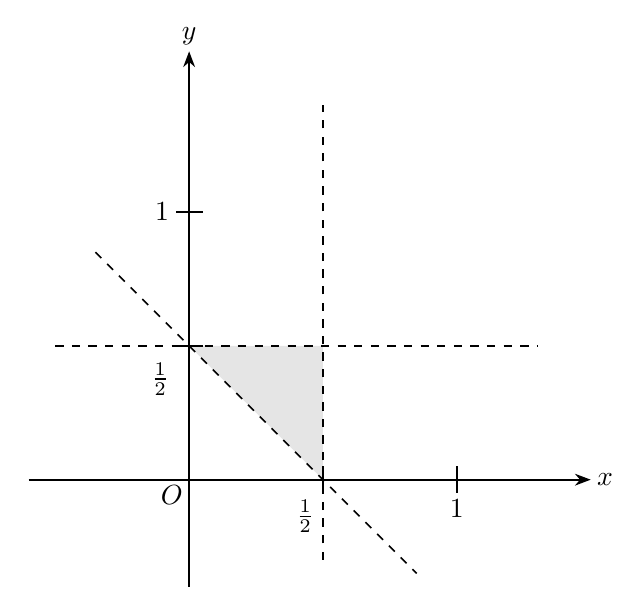
\begin{tikzpicture}[x=3.4cm,y=3.4cm,line width=.6pt,font=\normalsize,every node/.style={inner sep=0pt},>=Stealth]
% shaded feasible triangle (0,1/2)-(1/2,1/2)-(1/2,0)
\fill[gray!20,draw=none] (0,0.5) -- (0.5,0.5) -- (0.5,0) -- cycle;
% dashed boundaries
\draw[dashed] (-0.5,0.5) -- (1.3,0.5);
\draw[dashed] (0.5,-0.3) -- (0.5,1.4);
\draw[dashed] (-0.35,0.85) -- (0.85,-0.35);
% axes (over last tick 1 by half grid 0.5)
\draw[->] (-0.6,0) -- (1.5,0);
\draw[->] (0,-0.4) -- (0,1.6);
% ticks
\draw (0.5,0.05) -- (0.5,-0.05);
\draw (1,0.05) -- (1,-0.05);
\draw (0.05,0.5) -- (-0.05,0.5);
\draw (0.05,1) -- (-0.05,1);
% tick numerals (2pt clear, no white fill)
\node[below left,inner sep=0pt,xshift=-3pt,yshift=-7pt] at (0.5,0) {$\frac{1}{2}$};
\node[below=7pt,inner sep=0pt] at (1,0) {$1$};
\node[left=7pt,inner sep=0pt,yshift=-12pt] at (0,0.5) {$\frac{1}{2}$};
\node[left=7pt,inner sep=0pt] at (0,1) {$1$};
% axis labels outside arrows
\node[below left,inner sep=0pt,xshift=-2pt,yshift=-2pt] at (0,0) {$O$};
\node[right=2pt,inner sep=0pt] at (1.5,0) {$x$};
\node[above=2pt,inner sep=0pt] at (0,1.6) {$y$};
\end{tikzpicture}
